\documentclass[twoside]{book}

% Packages required by doxygen
\usepackage{fixltx2e}
\usepackage{calc}
\usepackage{doxygen}
\usepackage{graphicx}
\usepackage[utf8]{inputenc}
\usepackage{makeidx}
\usepackage{multicol}
\usepackage{multirow}
\PassOptionsToPackage{warn}{textcomp}
\usepackage{textcomp}
\usepackage[nointegrals]{wasysym}
\usepackage[table]{xcolor}

% Font selection
\usepackage[T1]{fontenc}
\usepackage{mathptmx}
\usepackage[scaled=.90]{helvet}
\usepackage{courier}
\usepackage{amssymb}
\usepackage{sectsty}
\renewcommand{\familydefault}{\sfdefault}
\allsectionsfont{%
  \fontseries{bc}\selectfont%
  \color{darkgray}%
}
\renewcommand{\DoxyLabelFont}{%
  \fontseries{bc}\selectfont%
  \color{darkgray}%
}
\newcommand{\+}{\discretionary{\mbox{\scriptsize$\hookleftarrow$}}{}{}}

% Page & text layout
\usepackage{geometry}
\geometry{%
  a4paper,%
  top=2.5cm,%
  bottom=2.5cm,%
  left=2.5cm,%
  right=2.5cm%
}
\tolerance=750
\hfuzz=15pt
\hbadness=750
\setlength{\emergencystretch}{15pt}
\setlength{\parindent}{0cm}
\setlength{\parskip}{0.2cm}
\makeatletter
\renewcommand{\paragraph}{%
  \@startsection{paragraph}{4}{0ex}{-1.0ex}{1.0ex}{%
    \normalfont\normalsize\bfseries\SS@parafont%
  }%
}
\renewcommand{\subparagraph}{%
  \@startsection{subparagraph}{5}{0ex}{-1.0ex}{1.0ex}{%
    \normalfont\normalsize\bfseries\SS@subparafont%
  }%
}
\makeatother

% Headers & footers
\usepackage{fancyhdr}
\pagestyle{fancyplain}
\fancyhead[LE]{\fancyplain{}{\bfseries\thepage}}
\fancyhead[CE]{\fancyplain{}{}}
\fancyhead[RE]{\fancyplain{}{\bfseries\leftmark}}
\fancyhead[LO]{\fancyplain{}{\bfseries\rightmark}}
\fancyhead[CO]{\fancyplain{}{}}
\fancyhead[RO]{\fancyplain{}{\bfseries\thepage}}
\fancyfoot[LE]{\fancyplain{}{}}
\fancyfoot[CE]{\fancyplain{}{}}
\fancyfoot[RE]{\fancyplain{}{\bfseries\scriptsize Generated on Wed Sep 28 2016 01\+:58\+:59 for Laboratorio\+\_\+2 by Doxygen }}
\fancyfoot[LO]{\fancyplain{}{\bfseries\scriptsize Generated on Wed Sep 28 2016 01\+:58\+:59 for Laboratorio\+\_\+2 by Doxygen }}
\fancyfoot[CO]{\fancyplain{}{}}
\fancyfoot[RO]{\fancyplain{}{}}
\renewcommand{\footrulewidth}{0.4pt}
\renewcommand{\chaptermark}[1]{%
  \markboth{#1}{}%
}
\renewcommand{\sectionmark}[1]{%
  \markright{\thesection\ #1}%
}

% Indices & bibliography
\usepackage{natbib}
\usepackage[titles]{tocloft}
\setcounter{tocdepth}{3}
\setcounter{secnumdepth}{5}
\makeindex

% Hyperlinks (required, but should be loaded last)
\usepackage{ifpdf}
\ifpdf
  \usepackage[pdftex,pagebackref=true]{hyperref}
\else
  \usepackage[ps2pdf,pagebackref=true]{hyperref}
\fi
\hypersetup{%
  colorlinks=true,%
  linkcolor=blue,%
  citecolor=blue,%
  unicode%
}

% Custom commands
\newcommand{\clearemptydoublepage}{%
  \newpage{\pagestyle{empty}\cleardoublepage}%
}


%===== C O N T E N T S =====

\begin{document}

% Titlepage & ToC
\hypersetup{pageanchor=false,
             bookmarks=true,
             bookmarksnumbered=true,
             pdfencoding=unicode
            }
\pagenumbering{roman}
\begin{titlepage}
\vspace*{7cm}
\begin{center}%
{\Large Laboratorio\+\_\+2 \\[1ex]\large 1.\+0 }\\
\vspace*{1cm}
{\large Generated by Doxygen 1.8.8}\\
\vspace*{0.5cm}
{\small Wed Sep 28 2016 01:58:59}\\
\end{center}
\end{titlepage}
\clearemptydoublepage
\tableofcontents
\clearemptydoublepage
\pagenumbering{arabic}
\hypersetup{pageanchor=true}

%--- Begin generated contents ---
\chapter{Herencia, poliformísmo y sobrecargas en C++}
\label{index}\hypertarget{index}{}\begin{DoxyAuthor}{Author}
Dunia Barahona \href{mailto:s4si@hotmail.com}{\tt s4si@hotmail.\+com} 
\end{DoxyAuthor}
\begin{DoxyDate}{Date}
11 de setiembre de 2016 
\end{DoxyDate}
\begin{DoxyVersion}{Version}
1.\+0 
\end{DoxyVersion}
\begin{DoxyParagraph}{Descripción}
Serie de clases que modelan figuras geométricas. La clase base se llama \hyperlink{class_figura}{Figura} y las derivadas son \hyperlink{class_circulo}{Circulo}, \hyperlink{class_cuadrado}{Cuadrado} y \hyperlink{class_triangulo}{Triangulo}; cada una tiene su respectivo archivo de encabezados. Todas estas clases estan implementadas en el \hyperlink{main_8cpp_a3c04138a5bfe5d72780bb7e82a18e627}{main} . 
\end{DoxyParagraph}

\chapter{Hierarchical Index}
\section{Class Hierarchy}
This inheritance list is sorted roughly, but not completely, alphabetically\+:\begin{DoxyCompactList}
\item \contentsline{section}{Figura}{\pageref{class_figura}}{}
\begin{DoxyCompactList}
\item \contentsline{section}{Circulo}{\pageref{class_circulo}}{}
\item \contentsline{section}{Cuadrado}{\pageref{class_cuadrado}}{}
\item \contentsline{section}{Triangulo}{\pageref{class_triangulo}}{}
\end{DoxyCompactList}
\end{DoxyCompactList}

\chapter{Class Index}
\section{Class List}
Here are the classes, structs, unions and interfaces with brief descriptions\+:\begin{DoxyCompactList}
\item\contentsline{section}{\hyperlink{class_calculadora}{Calculadora$<$ data $>$} }{\pageref{class_calculadora}}{}
\item\contentsline{section}{\hyperlink{class_fraccion}{Fraccion} }{\pageref{class_fraccion}}{}
\item\contentsline{section}{\hyperlink{class_matriz}{Matriz} }{\pageref{class_matriz}}{}
\item\contentsline{section}{\hyperlink{class_polinomio}{Polinomio} }{\pageref{class_polinomio}}{}
\end{DoxyCompactList}

\chapter{File Index}
\section{File List}
Here is a list of all files with brief descriptions\+:\begin{DoxyCompactList}
\item\contentsline{section}{\hyperlink{_circulo_8cpp}{Circulo.\+cpp} }{\pageref{_circulo_8cpp}}{}
\item\contentsline{section}{\hyperlink{_circulo_8h}{Circulo.\+h} }{\pageref{_circulo_8h}}{}
\item\contentsline{section}{\hyperlink{_cuadrado_8cpp}{Cuadrado.\+cpp} }{\pageref{_cuadrado_8cpp}}{}
\item\contentsline{section}{\hyperlink{_cuadrado_8h}{Cuadrado.\+h} }{\pageref{_cuadrado_8h}}{}
\item\contentsline{section}{\hyperlink{_figura_8cpp}{Figura.\+cpp} }{\pageref{_figura_8cpp}}{}
\item\contentsline{section}{\hyperlink{_figura_8h}{Figura.\+h} }{\pageref{_figura_8h}}{}
\item\contentsline{section}{\hyperlink{main_8cpp}{main.\+cpp} }{\pageref{main_8cpp}}{}
\item\contentsline{section}{\hyperlink{_triangulo_8cpp}{Triangulo.\+cpp} }{\pageref{_triangulo_8cpp}}{}
\item\contentsline{section}{\hyperlink{_triangulo_8h}{Triangulo.\+h} }{\pageref{_triangulo_8h}}{}
\end{DoxyCompactList}

\chapter{Class Documentation}
\hypertarget{class_circulo}{\section{Circulo Class Reference}
\label{class_circulo}\index{Circulo@{Circulo}}
}


Hereda de la clase \hyperlink{class_figura}{Figura} .  




{\ttfamily \#include $<$Circulo.\+h$>$}



Inheritance diagram for Circulo\+:
\nopagebreak
\begin{figure}[H]
\begin{center}
\leavevmode
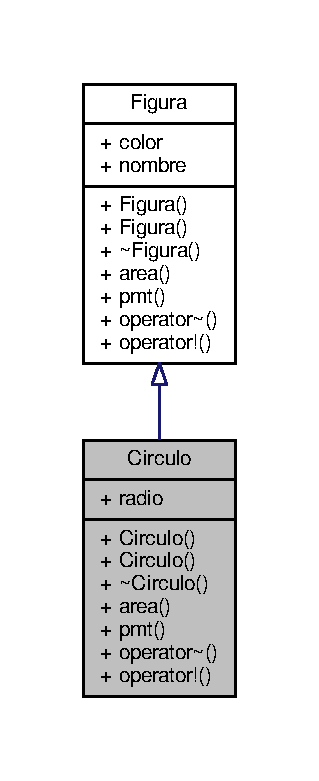
\includegraphics[width=153pt]{class_circulo__inherit__graph}
\end{center}
\end{figure}
\subsection*{Public Member Functions}
\begin{DoxyCompactItemize}
\item 
\hyperlink{class_circulo_a6933bf908b78a4167684081a3a8f257f}{Circulo} ()
\item 
\hyperlink{class_circulo_a14db1f1a04f7adfa9f3e785fce82419c}{Circulo} (string \hyperlink{class_figura_a5be336617ed8a4d4f28115297b38da02}{nombre}, string \hyperlink{class_figura_a9f519b9504b95440f124a3099070e952}{color}, double \hyperlink{class_circulo_aba57029c5768d344c4ef536e5323122b}{radio})
\item 
virtual \hyperlink{class_circulo_a8efe39e0e89487519cd802f0738d3bf4}{$\sim$\+Circulo} ()
\item 
virtual double \hyperlink{class_circulo_aded0c4ee374eb000f59d8d8da01ad72d}{area} ()
\item 
virtual double \hyperlink{class_circulo_afd102e74c7b2c368979f8ad042a02805}{pmt} ()
\item 
virtual void \hyperlink{class_circulo_a8db226b0c3bad5b8a01d60afb45838c7}{operator$\sim$} ()
\item 
virtual void \hyperlink{class_circulo_a64bd2cabfdbca872d44bf1eb13f59cbb}{operator!} ()
\end{DoxyCompactItemize}
\subsection*{Public Attributes}
\begin{DoxyCompactItemize}
\item 
double \hyperlink{class_circulo_aba57029c5768d344c4ef536e5323122b}{radio}
\begin{DoxyCompactList}\small\item\em Corresponde al radio del círculo. \end{DoxyCompactList}\end{DoxyCompactItemize}


\subsection{Detailed Description}
Hereda de la clase \hyperlink{class_figura}{Figura} . 

\subsection{Constructor \& Destructor Documentation}
\hypertarget{class_circulo_a6933bf908b78a4167684081a3a8f257f}{\index{Circulo@{Circulo}!Circulo@{Circulo}}
\index{Circulo@{Circulo}!Circulo@{Circulo}}
\subsubsection[{Circulo}]{\setlength{\rightskip}{0pt plus 5cm}Circulo\+::\+Circulo (
\begin{DoxyParamCaption}
{}
\end{DoxyParamCaption}
)}}\label{class_circulo_a6933bf908b78a4167684081a3a8f257f}
El {\bfseries constructor} es una función que se llama igual que la clase. \hypertarget{class_circulo_a14db1f1a04f7adfa9f3e785fce82419c}{\index{Circulo@{Circulo}!Circulo@{Circulo}}
\index{Circulo@{Circulo}!Circulo@{Circulo}}
\subsubsection[{Circulo}]{\setlength{\rightskip}{0pt plus 5cm}Circulo\+::\+Circulo (
\begin{DoxyParamCaption}
\item[{string}]{nombre, }
\item[{string}]{color, }
\item[{double}]{radio}
\end{DoxyParamCaption}
)}}\label{class_circulo_a14db1f1a04f7adfa9f3e785fce82419c}
Constructor que recibe los atributos como parámetros. \hypertarget{class_circulo_a8efe39e0e89487519cd802f0738d3bf4}{\index{Circulo@{Circulo}!````~Circulo@{$\sim$\+Circulo}}
\index{````~Circulo@{$\sim$\+Circulo}!Circulo@{Circulo}}
\subsubsection[{$\sim$\+Circulo}]{\setlength{\rightskip}{0pt plus 5cm}Circulo\+::$\sim$\+Circulo (
\begin{DoxyParamCaption}
{}
\end{DoxyParamCaption}
)\hspace{0.3cm}{\ttfamily [virtual]}}}\label{class_circulo_a8efe39e0e89487519cd802f0738d3bf4}
Destructor, sirve para destruir un objeto de la clase. 

\subsection{Member Function Documentation}
\hypertarget{class_circulo_aded0c4ee374eb000f59d8d8da01ad72d}{\index{Circulo@{Circulo}!area@{area}}
\index{area@{area}!Circulo@{Circulo}}
\subsubsection[{area}]{\setlength{\rightskip}{0pt plus 5cm}double Circulo\+::area (
\begin{DoxyParamCaption}
{}
\end{DoxyParamCaption}
)\hspace{0.3cm}{\ttfamily [virtual]}}}\label{class_circulo_aded0c4ee374eb000f59d8d8da01ad72d}
Calcula el área del círculo dado su radio como atributo del objeto. \begin{DoxyReturn}{Returns}
Área del círculo. 
\end{DoxyReturn}


Reimplemented from \hyperlink{class_figura_ade6b12995c86cb72e37738668d77963d}{Figura}.

\hypertarget{class_circulo_a64bd2cabfdbca872d44bf1eb13f59cbb}{\index{Circulo@{Circulo}!operator"!@{operator"!}}
\index{operator"!@{operator"!}!Circulo@{Circulo}}
\subsubsection[{operator"!}]{\setlength{\rightskip}{0pt plus 5cm}void Circulo\+::operator! (
\begin{DoxyParamCaption}
{}
\end{DoxyParamCaption}
)\hspace{0.3cm}{\ttfamily [virtual]}}}\label{class_circulo_a64bd2cabfdbca872d44bf1eb13f59cbb}
Sobrecarga del operador {\bfseries !} 

Imprime los valores calculados del área y perímetro del círculo. 

Reimplemented from \hyperlink{class_figura_a361ecd93374af526d5b791b7b67d510a}{Figura}.

\hypertarget{class_circulo_a8db226b0c3bad5b8a01d60afb45838c7}{\index{Circulo@{Circulo}!operator````~@{operator$\sim$}}
\index{operator````~@{operator$\sim$}!Circulo@{Circulo}}
\subsubsection[{operator$\sim$}]{\setlength{\rightskip}{0pt plus 5cm}void Circulo\+::operator$\sim$ (
\begin{DoxyParamCaption}
{}
\end{DoxyParamCaption}
)\hspace{0.3cm}{\ttfamily [virtual]}}}\label{class_circulo_a8db226b0c3bad5b8a01d60afb45838c7}
Sobrecarga del operador {\bfseries $\sim$} 

Imprime los atributos del objeto. 

Reimplemented from \hyperlink{class_figura_ab0e96a77be9c277b66b7ae73172fdcb0}{Figura}.

\hypertarget{class_circulo_afd102e74c7b2c368979f8ad042a02805}{\index{Circulo@{Circulo}!pmt@{pmt}}
\index{pmt@{pmt}!Circulo@{Circulo}}
\subsubsection[{pmt}]{\setlength{\rightskip}{0pt plus 5cm}double Circulo\+::pmt (
\begin{DoxyParamCaption}
{}
\end{DoxyParamCaption}
)\hspace{0.3cm}{\ttfamily [virtual]}}}\label{class_circulo_afd102e74c7b2c368979f8ad042a02805}
Calcula el perímetro del círculo dado su radio como atributo del objeto. \begin{DoxyReturn}{Returns}
Perímetro del círculo. 
\end{DoxyReturn}


Reimplemented from \hyperlink{class_figura_a522ea732b30ffa838731fced76a593ef}{Figura}.



\subsection{Member Data Documentation}
\hypertarget{class_circulo_aba57029c5768d344c4ef536e5323122b}{\index{Circulo@{Circulo}!radio@{radio}}
\index{radio@{radio}!Circulo@{Circulo}}
\subsubsection[{radio}]{\setlength{\rightskip}{0pt plus 5cm}double Circulo\+::radio}}\label{class_circulo_aba57029c5768d344c4ef536e5323122b}


Corresponde al radio del círculo. 



The documentation for this class was generated from the following files\+:\begin{DoxyCompactItemize}
\item 
code/\hyperlink{_circulo_8h}{Circulo.\+h}\item 
code/\hyperlink{_circulo_8cpp}{Circulo.\+cpp}\end{DoxyCompactItemize}

\hypertarget{class_cuadrado}{\section{Cuadrado Class Reference}
\label{class_cuadrado}\index{Cuadrado@{Cuadrado}}
}


Hereda de la clase \hyperlink{class_figura}{Figura} .  




{\ttfamily \#include $<$Cuadrado.\+h$>$}



Inheritance diagram for Cuadrado\+:\nopagebreak
\begin{figure}[H]
\begin{center}
\leavevmode
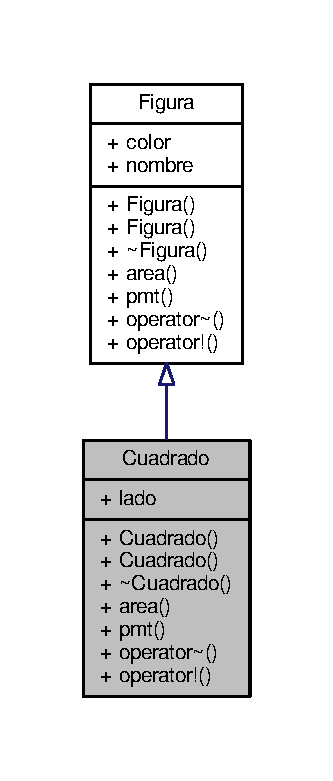
\includegraphics[width=160pt]{class_cuadrado__inherit__graph}
\end{center}
\end{figure}
\subsection*{Public Member Functions}
\begin{DoxyCompactItemize}
\item 
\hyperlink{class_cuadrado_ad28d9dddc29e1987ec620b07b0a4acc9}{Cuadrado} ()
\item 
\hyperlink{class_cuadrado_afb489ccf7f7b4e2837d080bee5f6656a}{Cuadrado} (string \hyperlink{class_figura_a5be336617ed8a4d4f28115297b38da02}{nombre}, string \hyperlink{class_figura_a9f519b9504b95440f124a3099070e952}{color}, double \hyperlink{class_cuadrado_a0480679f3e1c059282f532167c81d439}{lado})
\item 
virtual \hyperlink{class_cuadrado_a9f5bf29c9b8368ad45a4a3c12f9fd7c2}{$\sim$\+Cuadrado} ()
\item 
virtual double \hyperlink{class_cuadrado_a379a755de0b95f295e30e6049e19426c}{area} ()
\item 
virtual double \hyperlink{class_cuadrado_ace7ee6909f89aeb0797a135a03be4fe4}{pmt} ()
\item 
virtual void \hyperlink{class_cuadrado_a6303f81de8d357f415d00a116b73a6fc}{operator$\sim$} ()
\item 
virtual void \hyperlink{class_cuadrado_a78be5dcef640ad7f82858f44fb623af5}{operator!} ()
\end{DoxyCompactItemize}
\subsection*{Public Attributes}
\begin{DoxyCompactItemize}
\item 
double \hyperlink{class_cuadrado_a0480679f3e1c059282f532167c81d439}{lado}
\begin{DoxyCompactList}\small\item\em Corresponde a la longitud de lado del cuadrado. \end{DoxyCompactList}\end{DoxyCompactItemize}


\subsection{Detailed Description}
Hereda de la clase \hyperlink{class_figura}{Figura} . 

\subsection{Constructor \& Destructor Documentation}
\hypertarget{class_cuadrado_ad28d9dddc29e1987ec620b07b0a4acc9}{\index{Cuadrado@{Cuadrado}!Cuadrado@{Cuadrado}}
\index{Cuadrado@{Cuadrado}!Cuadrado@{Cuadrado}}
\subsubsection[{Cuadrado}]{\setlength{\rightskip}{0pt plus 5cm}Cuadrado\+::\+Cuadrado (
\begin{DoxyParamCaption}
{}
\end{DoxyParamCaption}
)}}\label{class_cuadrado_ad28d9dddc29e1987ec620b07b0a4acc9}
El {\bfseries constructor} es un método que se llama igual que la clase. \hypertarget{class_cuadrado_afb489ccf7f7b4e2837d080bee5f6656a}{\index{Cuadrado@{Cuadrado}!Cuadrado@{Cuadrado}}
\index{Cuadrado@{Cuadrado}!Cuadrado@{Cuadrado}}
\subsubsection[{Cuadrado}]{\setlength{\rightskip}{0pt plus 5cm}Cuadrado\+::\+Cuadrado (
\begin{DoxyParamCaption}
\item[{string}]{nombre, }
\item[{string}]{color, }
\item[{double}]{lado}
\end{DoxyParamCaption}
)}}\label{class_cuadrado_afb489ccf7f7b4e2837d080bee5f6656a}
Constructor que recibe los atributos como parámetros. \hypertarget{class_cuadrado_a9f5bf29c9b8368ad45a4a3c12f9fd7c2}{\index{Cuadrado@{Cuadrado}!````~Cuadrado@{$\sim$\+Cuadrado}}
\index{````~Cuadrado@{$\sim$\+Cuadrado}!Cuadrado@{Cuadrado}}
\subsubsection[{$\sim$\+Cuadrado}]{\setlength{\rightskip}{0pt plus 5cm}Cuadrado\+::$\sim$\+Cuadrado (
\begin{DoxyParamCaption}
{}
\end{DoxyParamCaption}
)\hspace{0.3cm}{\ttfamily [virtual]}}}\label{class_cuadrado_a9f5bf29c9b8368ad45a4a3c12f9fd7c2}
Destructor, sirve para destruir un objeto de la clase. 

\subsection{Member Function Documentation}
\hypertarget{class_cuadrado_a379a755de0b95f295e30e6049e19426c}{\index{Cuadrado@{Cuadrado}!area@{area}}
\index{area@{area}!Cuadrado@{Cuadrado}}
\subsubsection[{area}]{\setlength{\rightskip}{0pt plus 5cm}double Cuadrado\+::area (
\begin{DoxyParamCaption}
{}
\end{DoxyParamCaption}
)\hspace{0.3cm}{\ttfamily [virtual]}}}\label{class_cuadrado_a379a755de0b95f295e30e6049e19426c}
Calcula el área del cuadrado dada la longitud de lado como atributo del objeto. \begin{DoxyReturn}{Returns}
Área del cuadrado. 
\end{DoxyReturn}


Reimplemented from \hyperlink{class_figura_ade6b12995c86cb72e37738668d77963d}{Figura}.

\hypertarget{class_cuadrado_a78be5dcef640ad7f82858f44fb623af5}{\index{Cuadrado@{Cuadrado}!operator"!@{operator"!}}
\index{operator"!@{operator"!}!Cuadrado@{Cuadrado}}
\subsubsection[{operator"!}]{\setlength{\rightskip}{0pt plus 5cm}void Cuadrado\+::operator! (
\begin{DoxyParamCaption}
{}
\end{DoxyParamCaption}
)\hspace{0.3cm}{\ttfamily [virtual]}}}\label{class_cuadrado_a78be5dcef640ad7f82858f44fb623af5}
Sobrecarga del operador {\bfseries !} 

Imprime los valores calculados del área y perímetro del cuadrado. 

Reimplemented from \hyperlink{class_figura_a361ecd93374af526d5b791b7b67d510a}{Figura}.

\hypertarget{class_cuadrado_a6303f81de8d357f415d00a116b73a6fc}{\index{Cuadrado@{Cuadrado}!operator````~@{operator$\sim$}}
\index{operator````~@{operator$\sim$}!Cuadrado@{Cuadrado}}
\subsubsection[{operator$\sim$}]{\setlength{\rightskip}{0pt plus 5cm}void Cuadrado\+::operator$\sim$ (
\begin{DoxyParamCaption}
{}
\end{DoxyParamCaption}
)\hspace{0.3cm}{\ttfamily [virtual]}}}\label{class_cuadrado_a6303f81de8d357f415d00a116b73a6fc}
Sobrecarga del operador {\bfseries $\sim$} 

Imprime los atributos del objeto. 

Reimplemented from \hyperlink{class_figura_ab0e96a77be9c277b66b7ae73172fdcb0}{Figura}.

\hypertarget{class_cuadrado_ace7ee6909f89aeb0797a135a03be4fe4}{\index{Cuadrado@{Cuadrado}!pmt@{pmt}}
\index{pmt@{pmt}!Cuadrado@{Cuadrado}}
\subsubsection[{pmt}]{\setlength{\rightskip}{0pt plus 5cm}double Cuadrado\+::pmt (
\begin{DoxyParamCaption}
{}
\end{DoxyParamCaption}
)\hspace{0.3cm}{\ttfamily [virtual]}}}\label{class_cuadrado_ace7ee6909f89aeb0797a135a03be4fe4}
Calcula el perímetro del cuadrado dada la longitud de lado como atributo del objeto. \begin{DoxyReturn}{Returns}
Perímetro del cuadrado. 
\end{DoxyReturn}


Reimplemented from \hyperlink{class_figura_a522ea732b30ffa838731fced76a593ef}{Figura}.



\subsection{Member Data Documentation}
\hypertarget{class_cuadrado_a0480679f3e1c059282f532167c81d439}{\index{Cuadrado@{Cuadrado}!lado@{lado}}
\index{lado@{lado}!Cuadrado@{Cuadrado}}
\subsubsection[{lado}]{\setlength{\rightskip}{0pt plus 5cm}double Cuadrado\+::lado}}\label{class_cuadrado_a0480679f3e1c059282f532167c81d439}


Corresponde a la longitud de lado del cuadrado. 



The documentation for this class was generated from the following files\+:\begin{DoxyCompactItemize}
\item 
code/\hyperlink{_cuadrado_8h}{Cuadrado.\+h}\item 
code/\hyperlink{_cuadrado_8cpp}{Cuadrado.\+cpp}\end{DoxyCompactItemize}

\hypertarget{class_figura}{\section{Figura Class Reference}
\label{class_figura}\index{Figura@{Figura}}
}


Clase base.  




{\ttfamily \#include $<$Figura.\+h$>$}



Inheritance diagram for Figura\+:\nopagebreak
\begin{figure}[H]
\begin{center}
\leavevmode
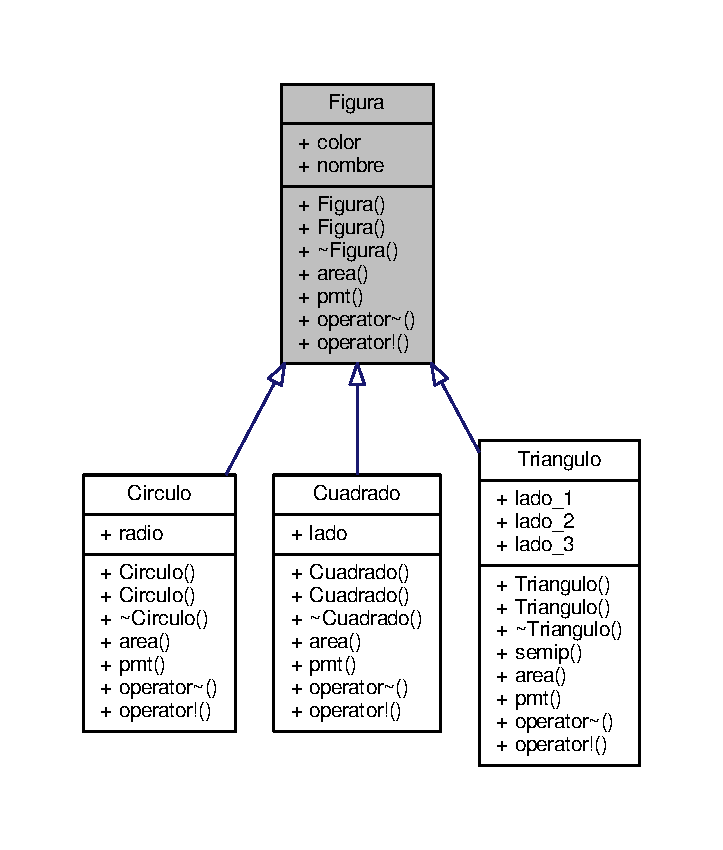
\includegraphics[width=347pt]{class_figura__inherit__graph}
\end{center}
\end{figure}
\subsection*{Public Member Functions}
\begin{DoxyCompactItemize}
\item 
\hyperlink{class_figura_a6977c7f0438c11b985a9a74c208b51c8}{Figura} ()
\item 
\hyperlink{class_figura_a35962837dabe47162c4f7549175f6f81}{Figura} (string \hyperlink{class_figura_a5be336617ed8a4d4f28115297b38da02}{nombre}, string \hyperlink{class_figura_a9f519b9504b95440f124a3099070e952}{color})
\item 
virtual \hyperlink{class_figura_a6130eb548893c36efcb7933e2da6821e}{$\sim$\+Figura} ()
\item 
virtual double \hyperlink{class_figura_ade6b12995c86cb72e37738668d77963d}{area} ()
\item 
virtual double \hyperlink{class_figura_a522ea732b30ffa838731fced76a593ef}{pmt} ()
\item 
virtual void \hyperlink{class_figura_ab0e96a77be9c277b66b7ae73172fdcb0}{operator$\sim$} ()
\item 
virtual void \hyperlink{class_figura_a361ecd93374af526d5b791b7b67d510a}{operator!} ()
\end{DoxyCompactItemize}
\subsection*{Public Attributes}
\begin{DoxyCompactItemize}
\item 
string \hyperlink{class_figura_a9f519b9504b95440f124a3099070e952}{color}
\begin{DoxyCompactList}\small\item\em Corresponde al color de la figura. \end{DoxyCompactList}\item 
string \hyperlink{class_figura_a5be336617ed8a4d4f28115297b38da02}{nombre}
\begin{DoxyCompactList}\small\item\em Corresponde al nombre de la figura. \end{DoxyCompactList}\end{DoxyCompactItemize}


\subsection{Detailed Description}
Clase base. 

\subsection{Constructor \& Destructor Documentation}
\hypertarget{class_figura_a6977c7f0438c11b985a9a74c208b51c8}{\index{Figura@{Figura}!Figura@{Figura}}
\index{Figura@{Figura}!Figura@{Figura}}
\subsubsection[{Figura}]{\setlength{\rightskip}{0pt plus 5cm}Figura\+::\+Figura (
\begin{DoxyParamCaption}
{}
\end{DoxyParamCaption}
)}}\label{class_figura_a6977c7f0438c11b985a9a74c208b51c8}
El {\bfseries constructor} es una función que se llama igual que la clase. \hypertarget{class_figura_a35962837dabe47162c4f7549175f6f81}{\index{Figura@{Figura}!Figura@{Figura}}
\index{Figura@{Figura}!Figura@{Figura}}
\subsubsection[{Figura}]{\setlength{\rightskip}{0pt plus 5cm}Figura\+::\+Figura (
\begin{DoxyParamCaption}
\item[{string}]{nombre, }
\item[{string}]{color}
\end{DoxyParamCaption}
)}}\label{class_figura_a35962837dabe47162c4f7549175f6f81}
Constructor que recibe los atributos como parámetros. \hypertarget{class_figura_a6130eb548893c36efcb7933e2da6821e}{\index{Figura@{Figura}!````~Figura@{$\sim$\+Figura}}
\index{````~Figura@{$\sim$\+Figura}!Figura@{Figura}}
\subsubsection[{$\sim$\+Figura}]{\setlength{\rightskip}{0pt plus 5cm}Figura\+::$\sim$\+Figura (
\begin{DoxyParamCaption}
{}
\end{DoxyParamCaption}
)\hspace{0.3cm}{\ttfamily [virtual]}}}\label{class_figura_a6130eb548893c36efcb7933e2da6821e}
Destructor, sirve para destruir un objeto de la clase. 

\subsection{Member Function Documentation}
\hypertarget{class_figura_ade6b12995c86cb72e37738668d77963d}{\index{Figura@{Figura}!area@{area}}
\index{area@{area}!Figura@{Figura}}
\subsubsection[{area}]{\setlength{\rightskip}{0pt plus 5cm}double Figura\+::area (
\begin{DoxyParamCaption}
{}
\end{DoxyParamCaption}
)\hspace{0.3cm}{\ttfamily [virtual]}}}\label{class_figura_ade6b12995c86cb72e37738668d77963d}
Función virtual que se reimplementa en las clases derivadas según cada caso. \begin{DoxyReturn}{Returns}
Área de la figura. 
\end{DoxyReturn}


Reimplemented in \hyperlink{class_triangulo_a1c71a04df8caa1bcb52898636fb20004}{Triangulo}, \hyperlink{class_circulo_aded0c4ee374eb000f59d8d8da01ad72d}{Circulo}, and \hyperlink{class_cuadrado_a379a755de0b95f295e30e6049e19426c}{Cuadrado}.

\hypertarget{class_figura_a361ecd93374af526d5b791b7b67d510a}{\index{Figura@{Figura}!operator"!@{operator"!}}
\index{operator"!@{operator"!}!Figura@{Figura}}
\subsubsection[{operator"!}]{\setlength{\rightskip}{0pt plus 5cm}void Figura\+::operator! (
\begin{DoxyParamCaption}
{}
\end{DoxyParamCaption}
)\hspace{0.3cm}{\ttfamily [virtual]}}}\label{class_figura_a361ecd93374af526d5b791b7b67d510a}
Sobrecarga del operador {\bfseries !} 

Imprime el mensaje correspondiente de los métodos \hyperlink{class_figura_ade6b12995c86cb72e37738668d77963d}{area} y \hyperlink{class_figura_a522ea732b30ffa838731fced76a593ef}{pmt} . 

Reimplemented in \hyperlink{class_triangulo_ae0552ffa9641d36e1f571349e5de1070}{Triangulo}, \hyperlink{class_circulo_a64bd2cabfdbca872d44bf1eb13f59cbb}{Circulo}, and \hyperlink{class_cuadrado_a78be5dcef640ad7f82858f44fb623af5}{Cuadrado}.

\hypertarget{class_figura_ab0e96a77be9c277b66b7ae73172fdcb0}{\index{Figura@{Figura}!operator````~@{operator$\sim$}}
\index{operator````~@{operator$\sim$}!Figura@{Figura}}
\subsubsection[{operator$\sim$}]{\setlength{\rightskip}{0pt plus 5cm}void Figura\+::operator$\sim$ (
\begin{DoxyParamCaption}
{}
\end{DoxyParamCaption}
)\hspace{0.3cm}{\ttfamily [virtual]}}}\label{class_figura_ab0e96a77be9c277b66b7ae73172fdcb0}
Sobrecarga del operador {\bfseries $\sim$} 

Imprime los atributos del objeto. 

Reimplemented in \hyperlink{class_triangulo_af7fc480161706ec74ece32e9ef1fed7f}{Triangulo}, \hyperlink{class_circulo_a8db226b0c3bad5b8a01d60afb45838c7}{Circulo}, and \hyperlink{class_cuadrado_a6303f81de8d357f415d00a116b73a6fc}{Cuadrado}.

\hypertarget{class_figura_a522ea732b30ffa838731fced76a593ef}{\index{Figura@{Figura}!pmt@{pmt}}
\index{pmt@{pmt}!Figura@{Figura}}
\subsubsection[{pmt}]{\setlength{\rightskip}{0pt plus 5cm}double Figura\+::pmt (
\begin{DoxyParamCaption}
{}
\end{DoxyParamCaption}
)\hspace{0.3cm}{\ttfamily [virtual]}}}\label{class_figura_a522ea732b30ffa838731fced76a593ef}
Función virtual que se reimplementa en las clases derivadas según cada caso. \begin{DoxyReturn}{Returns}
Perímetro de la figura. 
\end{DoxyReturn}


Reimplemented in \hyperlink{class_triangulo_ab82a50fa3dd74bc55606738ce5e31f7d}{Triangulo}, \hyperlink{class_circulo_afd102e74c7b2c368979f8ad042a02805}{Circulo}, and \hyperlink{class_cuadrado_ace7ee6909f89aeb0797a135a03be4fe4}{Cuadrado}.



\subsection{Member Data Documentation}
\hypertarget{class_figura_a9f519b9504b95440f124a3099070e952}{\index{Figura@{Figura}!color@{color}}
\index{color@{color}!Figura@{Figura}}
\subsubsection[{color}]{\setlength{\rightskip}{0pt plus 5cm}string Figura\+::color}}\label{class_figura_a9f519b9504b95440f124a3099070e952}


Corresponde al color de la figura. 

\hypertarget{class_figura_a5be336617ed8a4d4f28115297b38da02}{\index{Figura@{Figura}!nombre@{nombre}}
\index{nombre@{nombre}!Figura@{Figura}}
\subsubsection[{nombre}]{\setlength{\rightskip}{0pt plus 5cm}string Figura\+::nombre}}\label{class_figura_a5be336617ed8a4d4f28115297b38da02}


Corresponde al nombre de la figura. 



The documentation for this class was generated from the following files\+:\begin{DoxyCompactItemize}
\item 
code/\hyperlink{_figura_8h}{Figura.\+h}\item 
code/\hyperlink{_figura_8cpp}{Figura.\+cpp}\end{DoxyCompactItemize}

\hypertarget{class_triangulo}{\section{Triangulo Class Reference}
\label{class_triangulo}\index{Triangulo@{Triangulo}}
}


{\ttfamily \#include $<$Triangulo.\+h$>$}



Inheritance diagram for Triangulo\+:
\nopagebreak
\begin{figure}[H]
\begin{center}
\leavevmode
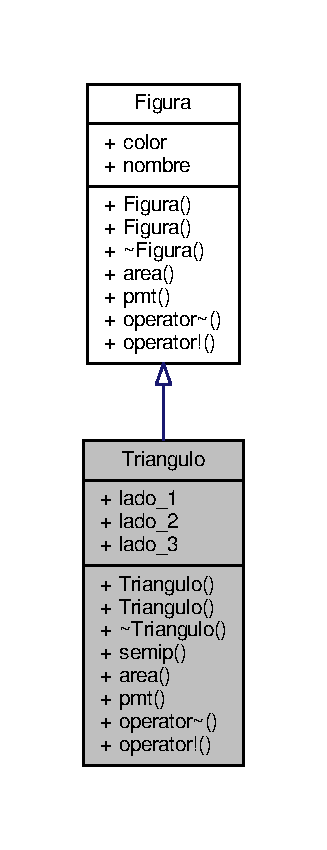
\includegraphics[width=157pt]{class_triangulo__inherit__graph}
\end{center}
\end{figure}


Collaboration diagram for Triangulo\+:
\nopagebreak
\begin{figure}[H]
\begin{center}
\leavevmode
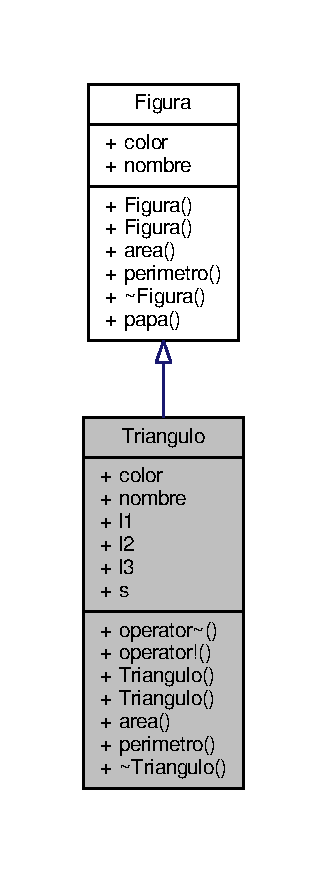
\includegraphics[width=157pt]{class_triangulo__coll__graph}
\end{center}
\end{figure}
\subsection*{Public Member Functions}
\begin{DoxyCompactItemize}
\item 
void \hyperlink{class_triangulo_af7fc480161706ec74ece32e9ef1fed7f}{operator$\sim$} ()
\begin{DoxyCompactList}\small\item\em Desplegador de los datos generales del triángulo. \end{DoxyCompactList}\item 
void \hyperlink{class_triangulo_ae0552ffa9641d36e1f571349e5de1070}{operator!} ()
\begin{DoxyCompactList}\small\item\em Desplegador del área y el perímetro del triángulo. \end{DoxyCompactList}\item 
\hyperlink{class_triangulo_a905d421bd19655a979ccad9e2998db0c}{Triangulo} ()
\begin{DoxyCompactList}\small\item\em Constructor de la clase triángulo. \end{DoxyCompactList}\item 
\hyperlink{class_triangulo_a5e645fd973d591e7c3d28bc74441787e}{Triangulo} (string \hyperlink{class_triangulo_a92bbfa4ca7bc38489e7bddd797a84cbf}{nombre}, string \hyperlink{class_triangulo_a437071d8f69923add54c5bedb74cce10}{color}, double \hyperlink{class_triangulo_a94ad3aafb95afd65f39dabc310b76209}{l1}, double \hyperlink{class_triangulo_a3aaa40dc5acbbd4079362c71a03cf016}{l2}, double \hyperlink{class_triangulo_aed89ff9f36a51cb7860f3175384c02eb}{l3})
\begin{DoxyCompactList}\small\item\em Constructor sobrecargado de la clase derivada triángulo. \end{DoxyCompactList}\item 
virtual double \hyperlink{class_triangulo_a1c71a04df8caa1bcb52898636fb20004}{area} ()
\begin{DoxyCompactList}\small\item\em Función general para cálculo de área de un triangulo. \end{DoxyCompactList}\item 
virtual double \hyperlink{class_triangulo_a6f5c542675a726b35f48f953bb2d9acf}{perimetro} ()
\begin{DoxyCompactList}\small\item\em Función general para cálculo de perímetro de un triangulo. \end{DoxyCompactList}\item 
virtual \hyperlink{class_triangulo_aca2be15b19831e8d7a5331808f5c1958}{$\sim$\+Triangulo} ()
\begin{DoxyCompactList}\small\item\em Destructor de la clase derivada triángulo. \end{DoxyCompactList}\end{DoxyCompactItemize}
\subsection*{Public Attributes}
\begin{DoxyCompactItemize}
\item 
string \hyperlink{class_triangulo_a437071d8f69923add54c5bedb74cce10}{color}
\item 
string \hyperlink{class_triangulo_a92bbfa4ca7bc38489e7bddd797a84cbf}{nombre}
\item 
double \hyperlink{class_triangulo_a94ad3aafb95afd65f39dabc310b76209}{l1}
\item 
double \hyperlink{class_triangulo_a3aaa40dc5acbbd4079362c71a03cf016}{l2}
\item 
double \hyperlink{class_triangulo_aed89ff9f36a51cb7860f3175384c02eb}{l3}
\item 
double \hyperlink{class_triangulo_a3a4640a5567d24a3df3c9f0462844ad8}{s}
\end{DoxyCompactItemize}


\subsection{Constructor \& Destructor Documentation}
\hypertarget{class_triangulo_a905d421bd19655a979ccad9e2998db0c}{\index{Triangulo@{Triangulo}!Triangulo@{Triangulo}}
\index{Triangulo@{Triangulo}!Triangulo@{Triangulo}}
\subsubsection[{Triangulo}]{\setlength{\rightskip}{0pt plus 5cm}Triangulo\+::\+Triangulo (
\begin{DoxyParamCaption}
{}
\end{DoxyParamCaption}
)}}\label{class_triangulo_a905d421bd19655a979ccad9e2998db0c}


Constructor de la clase triángulo. 

\hypertarget{class_triangulo_a5e645fd973d591e7c3d28bc74441787e}{\index{Triangulo@{Triangulo}!Triangulo@{Triangulo}}
\index{Triangulo@{Triangulo}!Triangulo@{Triangulo}}
\subsubsection[{Triangulo}]{\setlength{\rightskip}{0pt plus 5cm}Triangulo\+::\+Triangulo (
\begin{DoxyParamCaption}
\item[{string}]{nombre, }
\item[{string}]{color, }
\item[{double}]{l1, }
\item[{double}]{l2, }
\item[{double}]{l3}
\end{DoxyParamCaption}
)}}\label{class_triangulo_a5e645fd973d591e7c3d28bc74441787e}


Constructor sobrecargado de la clase derivada triángulo. 

\hypertarget{class_triangulo_aca2be15b19831e8d7a5331808f5c1958}{\index{Triangulo@{Triangulo}!````~Triangulo@{$\sim$\+Triangulo}}
\index{````~Triangulo@{$\sim$\+Triangulo}!Triangulo@{Triangulo}}
\subsubsection[{$\sim$\+Triangulo}]{\setlength{\rightskip}{0pt plus 5cm}Triangulo\+::$\sim$\+Triangulo (
\begin{DoxyParamCaption}
{}
\end{DoxyParamCaption}
)\hspace{0.3cm}{\ttfamily [virtual]}}}\label{class_triangulo_aca2be15b19831e8d7a5331808f5c1958}


Destructor de la clase derivada triángulo. 



\subsection{Member Function Documentation}
\hypertarget{class_triangulo_a1c71a04df8caa1bcb52898636fb20004}{\index{Triangulo@{Triangulo}!area@{area}}
\index{area@{area}!Triangulo@{Triangulo}}
\subsubsection[{area}]{\setlength{\rightskip}{0pt plus 5cm}double Triangulo\+::area (
\begin{DoxyParamCaption}
{}
\end{DoxyParamCaption}
)\hspace{0.3cm}{\ttfamily [virtual]}}}\label{class_triangulo_a1c71a04df8caa1bcb52898636fb20004}


Función general para cálculo de área de un triangulo. 



Reimplemented from \hyperlink{class_figura_ade6b12995c86cb72e37738668d77963d}{Figura}.



Here is the caller graph for this function\+:
\nopagebreak
\begin{figure}[H]
\begin{center}
\leavevmode
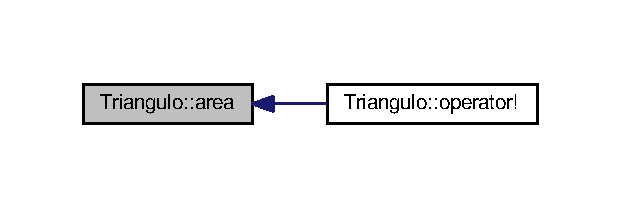
\includegraphics[width=298pt]{class_triangulo_a1c71a04df8caa1bcb52898636fb20004_icgraph}
\end{center}
\end{figure}


\hypertarget{class_triangulo_ae0552ffa9641d36e1f571349e5de1070}{\index{Triangulo@{Triangulo}!operator"!@{operator"!}}
\index{operator"!@{operator"!}!Triangulo@{Triangulo}}
\subsubsection[{operator"!}]{\setlength{\rightskip}{0pt plus 5cm}void Triangulo\+::operator! (
\begin{DoxyParamCaption}
{}
\end{DoxyParamCaption}
)}}\label{class_triangulo_ae0552ffa9641d36e1f571349e5de1070}


Desplegador del área y el perímetro del triángulo. 



Here is the call graph for this function\+:
\nopagebreak
\begin{figure}[H]
\begin{center}
\leavevmode
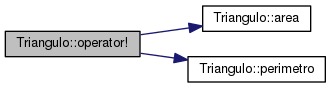
\includegraphics[width=320pt]{class_triangulo_ae0552ffa9641d36e1f571349e5de1070_cgraph}
\end{center}
\end{figure}


\hypertarget{class_triangulo_af7fc480161706ec74ece32e9ef1fed7f}{\index{Triangulo@{Triangulo}!operator````~@{operator$\sim$}}
\index{operator````~@{operator$\sim$}!Triangulo@{Triangulo}}
\subsubsection[{operator$\sim$}]{\setlength{\rightskip}{0pt plus 5cm}void Triangulo\+::operator$\sim$ (
\begin{DoxyParamCaption}
{}
\end{DoxyParamCaption}
)}}\label{class_triangulo_af7fc480161706ec74ece32e9ef1fed7f}


Desplegador de los datos generales del triángulo. 

\hypertarget{class_triangulo_a6f5c542675a726b35f48f953bb2d9acf}{\index{Triangulo@{Triangulo}!perimetro@{perimetro}}
\index{perimetro@{perimetro}!Triangulo@{Triangulo}}
\subsubsection[{perimetro}]{\setlength{\rightskip}{0pt plus 5cm}double Triangulo\+::perimetro (
\begin{DoxyParamCaption}
{}
\end{DoxyParamCaption}
)\hspace{0.3cm}{\ttfamily [virtual]}}}\label{class_triangulo_a6f5c542675a726b35f48f953bb2d9acf}


Función general para cálculo de perímetro de un triangulo. 



Reimplemented from \hyperlink{class_figura_a7451dfc1da3533fa15205df11afe7ac3}{Figura}.



Here is the caller graph for this function\+:
\nopagebreak
\begin{figure}[H]
\begin{center}
\leavevmode
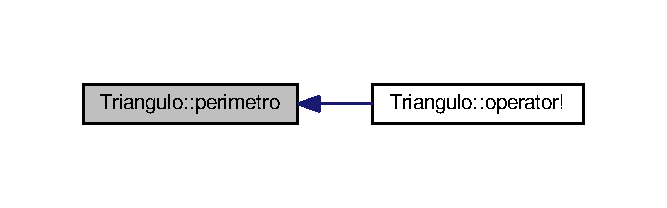
\includegraphics[width=320pt]{class_triangulo_a6f5c542675a726b35f48f953bb2d9acf_icgraph}
\end{center}
\end{figure}




\subsection{Member Data Documentation}
\hypertarget{class_triangulo_a437071d8f69923add54c5bedb74cce10}{\index{Triangulo@{Triangulo}!color@{color}}
\index{color@{color}!Triangulo@{Triangulo}}
\subsubsection[{color}]{\setlength{\rightskip}{0pt plus 5cm}string Triangulo\+::color}}\label{class_triangulo_a437071d8f69923add54c5bedb74cce10}
\hypertarget{class_triangulo_a94ad3aafb95afd65f39dabc310b76209}{\index{Triangulo@{Triangulo}!l1@{l1}}
\index{l1@{l1}!Triangulo@{Triangulo}}
\subsubsection[{l1}]{\setlength{\rightskip}{0pt plus 5cm}double Triangulo\+::l1}}\label{class_triangulo_a94ad3aafb95afd65f39dabc310b76209}
\hypertarget{class_triangulo_a3aaa40dc5acbbd4079362c71a03cf016}{\index{Triangulo@{Triangulo}!l2@{l2}}
\index{l2@{l2}!Triangulo@{Triangulo}}
\subsubsection[{l2}]{\setlength{\rightskip}{0pt plus 5cm}double Triangulo\+::l2}}\label{class_triangulo_a3aaa40dc5acbbd4079362c71a03cf016}
\hypertarget{class_triangulo_aed89ff9f36a51cb7860f3175384c02eb}{\index{Triangulo@{Triangulo}!l3@{l3}}
\index{l3@{l3}!Triangulo@{Triangulo}}
\subsubsection[{l3}]{\setlength{\rightskip}{0pt plus 5cm}double Triangulo\+::l3}}\label{class_triangulo_aed89ff9f36a51cb7860f3175384c02eb}
\hypertarget{class_triangulo_a92bbfa4ca7bc38489e7bddd797a84cbf}{\index{Triangulo@{Triangulo}!nombre@{nombre}}
\index{nombre@{nombre}!Triangulo@{Triangulo}}
\subsubsection[{nombre}]{\setlength{\rightskip}{0pt plus 5cm}string Triangulo\+::nombre}}\label{class_triangulo_a92bbfa4ca7bc38489e7bddd797a84cbf}
\hypertarget{class_triangulo_a3a4640a5567d24a3df3c9f0462844ad8}{\index{Triangulo@{Triangulo}!s@{s}}
\index{s@{s}!Triangulo@{Triangulo}}
\subsubsection[{s}]{\setlength{\rightskip}{0pt plus 5cm}double Triangulo\+::s}}\label{class_triangulo_a3a4640a5567d24a3df3c9f0462844ad8}


The documentation for this class was generated from the following files\+:\begin{DoxyCompactItemize}
\item 
\hyperlink{_triangulo_8h}{Triangulo.\+h}\item 
\hyperlink{_triangulo_8cpp}{Triangulo.\+cpp}\end{DoxyCompactItemize}

\chapter{File Documentation}
\hypertarget{_circulo_8cpp}{\section{code/\+Circulo.cpp File Reference}
\label{_circulo_8cpp}\index{code/\+Circulo.\+cpp@{code/\+Circulo.\+cpp}}
}
{\ttfamily \#include \char`\"{}Circulo.\+h\char`\"{}}\\*

\hypertarget{_circulo_8h}{\section{code/\+Circulo.h File Reference}
\label{_circulo_8h}\index{code/\+Circulo.\+h@{code/\+Circulo.\+h}}
}
{\ttfamily \#include \char`\"{}Figura.\+h\char`\"{}}\\*
\subsection*{Classes}
\begin{DoxyCompactItemize}
\item 
class \hyperlink{class_circulo}{Circulo}
\begin{DoxyCompactList}\small\item\em Hereda de la clase \hyperlink{class_figura}{Figura} . \end{DoxyCompactList}\end{DoxyCompactItemize}

\hypertarget{_cuadrado_8cpp}{\section{Cuadrado.\+cpp File Reference}
\label{_cuadrado_8cpp}\index{Cuadrado.\+cpp@{Cuadrado.\+cpp}}
}
{\ttfamily \#include \char`\"{}Figura.\+h\char`\"{}}\\*
{\ttfamily \#include \char`\"{}Cuadrado.\+h\char`\"{}}\\*
Include dependency graph for Cuadrado.\+cpp\+:
\nopagebreak
\begin{figure}[H]
\begin{center}
\leavevmode
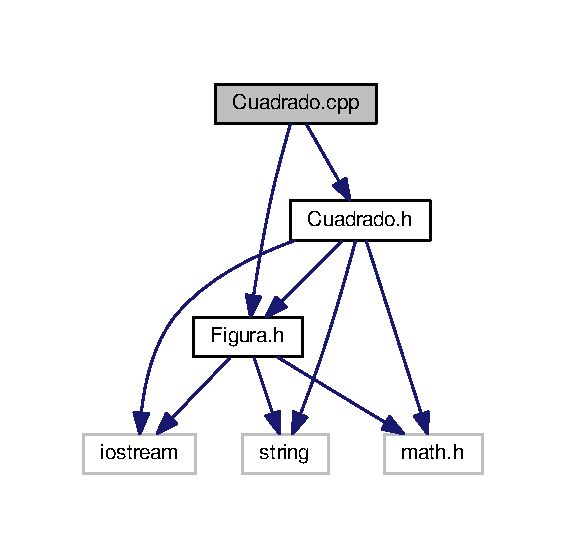
\includegraphics[width=272pt]{_cuadrado_8cpp__incl}
\end{center}
\end{figure}
\subsection*{Variables}
\begin{DoxyCompactItemize}
\item 
const double \hyperlink{_cuadrado_8cpp_a952eac791b596a61bba0a133a3bb439f}{P\+I} =3.\+141592653589793238463
\end{DoxyCompactItemize}


\subsection{Variable Documentation}
\hypertarget{_cuadrado_8cpp_a952eac791b596a61bba0a133a3bb439f}{\index{Cuadrado.\+cpp@{Cuadrado.\+cpp}!P\+I@{P\+I}}
\index{P\+I@{P\+I}!Cuadrado.\+cpp@{Cuadrado.\+cpp}}
\subsubsection[{P\+I}]{\setlength{\rightskip}{0pt plus 5cm}const double P\+I =3.\+141592653589793238463}}\label{_cuadrado_8cpp_a952eac791b596a61bba0a133a3bb439f}

\hypertarget{_cuadrado_8h}{\section{code/\+Cuadrado.h File Reference}
\label{_cuadrado_8h}\index{code/\+Cuadrado.\+h@{code/\+Cuadrado.\+h}}
}
{\ttfamily \#include \char`\"{}Figura.\+h\char`\"{}}\\*
\subsection*{Classes}
\begin{DoxyCompactItemize}
\item 
class \hyperlink{class_cuadrado}{Cuadrado}
\begin{DoxyCompactList}\small\item\em Hereda de la clase \hyperlink{class_figura}{Figura} . \end{DoxyCompactList}\end{DoxyCompactItemize}

\hypertarget{_figura_8cpp}{\section{Figura.\+cpp File Reference}
\label{_figura_8cpp}\index{Figura.\+cpp@{Figura.\+cpp}}
}
{\ttfamily \#include \char`\"{}Figura.\+h\char`\"{}}\\*
Include dependency graph for Figura.\+cpp\+:
\nopagebreak
\begin{figure}[H]
\begin{center}
\leavevmode
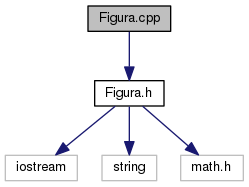
\includegraphics[width=259pt]{_figura_8cpp__incl}
\end{center}
\end{figure}

\hypertarget{_figura_8h}{\section{Figura.\+h File Reference}
\label{_figura_8h}\index{Figura.\+h@{Figura.\+h}}
}
{\ttfamily \#include $<$iostream$>$}\\*
{\ttfamily \#include \char`\"{}string\char`\"{}}\\*
{\ttfamily \#include $<$math.\+h$>$}\\*
Include dependency graph for Figura.\+h\+:
\nopagebreak
\begin{figure}[H]
\begin{center}
\leavevmode
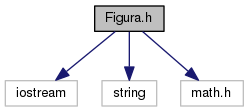
\includegraphics[width=259pt]{_figura_8h__incl}
\end{center}
\end{figure}
This graph shows which files directly or indirectly include this file\+:
\nopagebreak
\begin{figure}[H]
\begin{center}
\leavevmode
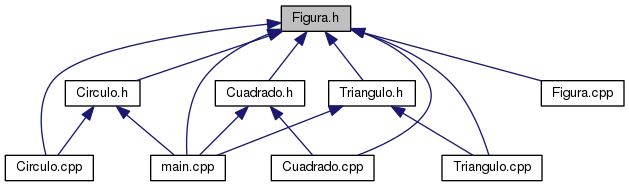
\includegraphics[width=350pt]{_figura_8h__dep__incl}
\end{center}
\end{figure}
\subsection*{Classes}
\begin{DoxyCompactItemize}
\item 
class \hyperlink{class_figura}{Figura}
\end{DoxyCompactItemize}

\hypertarget{main_8cpp}{\section{main.\+cpp File Reference}
\label{main_8cpp}\index{main.\+cpp@{main.\+cpp}}
}
{\ttfamily \#include $<$cstdlib$>$}\\*
{\ttfamily \#include \char`\"{}Node.\+h\char`\"{}}\\*
{\ttfamily \#include \char`\"{}Graph.\+h\char`\"{}}\\*
{\ttfamily \#include $<$queue$>$}\\*
Include dependency graph for main.\+cpp\+:\nopagebreak
\begin{figure}[H]
\begin{center}
\leavevmode
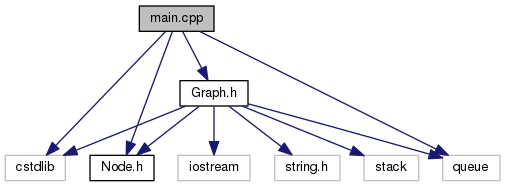
\includegraphics[width=350pt]{main_8cpp__incl}
\end{center}
\end{figure}
\subsection*{Macros}
\begin{DoxyCompactItemize}
\item 
\#define \hyperlink{main_8cpp_a4fc34b120ed3bd1120c1eb36abbcd6af}{N\+L}~cout $<$$<$ endl;
\item 
\#define \hyperlink{main_8cpp_aecd69d9a67487cc45c38eb184c50538a}{S\+P}~\char`\"{} \char`\"{}
\end{DoxyCompactItemize}
\subsection*{Functions}
\begin{DoxyCompactItemize}
\item 
int \hyperlink{main_8cpp_a3c04138a5bfe5d72780bb7e82a18e627}{main} (int argc, char $\ast$$\ast$argv)
\end{DoxyCompactItemize}


\subsection{Macro Definition Documentation}
\hypertarget{main_8cpp_a4fc34b120ed3bd1120c1eb36abbcd6af}{\index{main.\+cpp@{main.\+cpp}!N\+L@{N\+L}}
\index{N\+L@{N\+L}!main.\+cpp@{main.\+cpp}}
\subsubsection[{N\+L}]{\setlength{\rightskip}{0pt plus 5cm}\#define N\+L~cout $<$$<$ endl;}}\label{main_8cpp_a4fc34b120ed3bd1120c1eb36abbcd6af}
\hypertarget{main_8cpp_aecd69d9a67487cc45c38eb184c50538a}{\index{main.\+cpp@{main.\+cpp}!S\+P@{S\+P}}
\index{S\+P@{S\+P}!main.\+cpp@{main.\+cpp}}
\subsubsection[{S\+P}]{\setlength{\rightskip}{0pt plus 5cm}\#define S\+P~\char`\"{} \char`\"{}}}\label{main_8cpp_aecd69d9a67487cc45c38eb184c50538a}


\subsection{Function Documentation}
\hypertarget{main_8cpp_a3c04138a5bfe5d72780bb7e82a18e627}{\index{main.\+cpp@{main.\+cpp}!main@{main}}
\index{main@{main}!main.\+cpp@{main.\+cpp}}
\subsubsection[{main}]{\setlength{\rightskip}{0pt plus 5cm}int main (
\begin{DoxyParamCaption}
\item[{int}]{argc, }
\item[{char $\ast$$\ast$}]{argv}
\end{DoxyParamCaption}
)}}\label{main_8cpp_a3c04138a5bfe5d72780bb7e82a18e627}


Here is the call graph for this function\+:\nopagebreak
\begin{figure}[H]
\begin{center}
\leavevmode
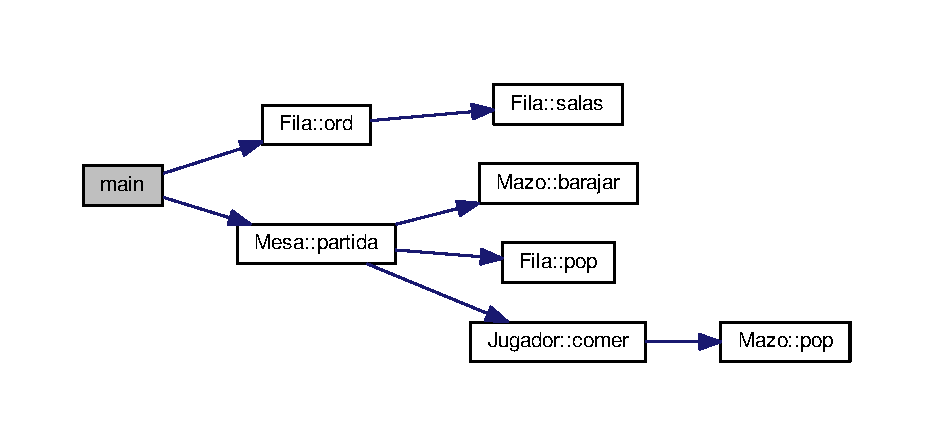
\includegraphics[width=240pt]{main_8cpp_a3c04138a5bfe5d72780bb7e82a18e627_cgraph}
\end{center}
\end{figure}



\hypertarget{_triangulo_8cpp}{\section{Triangulo.\+cpp File Reference}
\label{_triangulo_8cpp}\index{Triangulo.\+cpp@{Triangulo.\+cpp}}
}
{\ttfamily \#include \char`\"{}Triangulo.\+h\char`\"{}}\\*
{\ttfamily \#include \char`\"{}Figura.\+h\char`\"{}}\\*
Include dependency graph for Triangulo.\+cpp\+:
\nopagebreak
\begin{figure}[H]
\begin{center}
\leavevmode
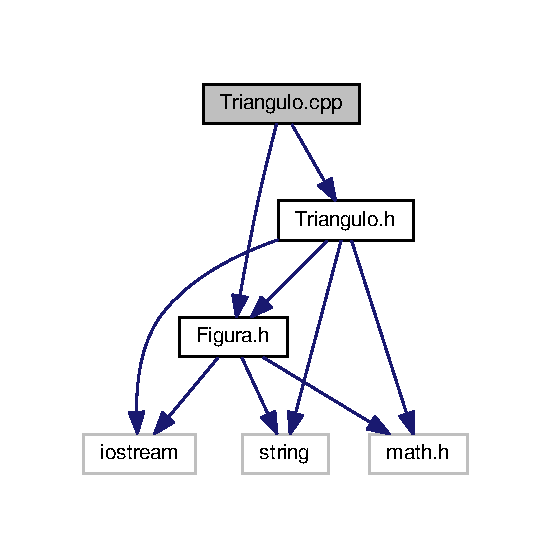
\includegraphics[width=265pt]{_triangulo_8cpp__incl}
\end{center}
\end{figure}

\hypertarget{_triangulo_8h}{\section{Triangulo.\+h File Reference}
\label{_triangulo_8h}\index{Triangulo.\+h@{Triangulo.\+h}}
}
{\ttfamily \#include $<$iostream$>$}\\*
{\ttfamily \#include \char`\"{}string\char`\"{}}\\*
{\ttfamily \#include \char`\"{}Figura.\+h\char`\"{}}\\*
{\ttfamily \#include $<$math.\+h$>$}\\*
Include dependency graph for Triangulo.\+h\+:
\nopagebreak
\begin{figure}[H]
\begin{center}
\leavevmode
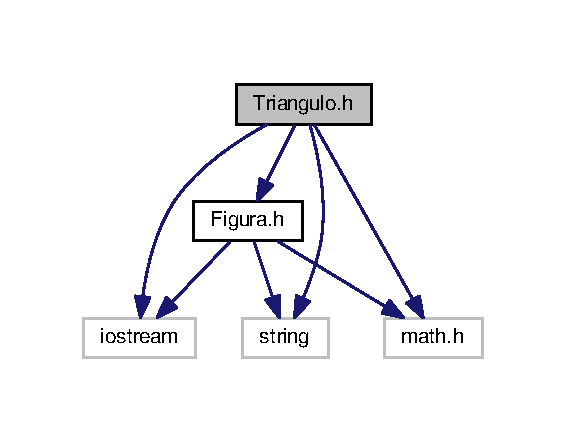
\includegraphics[width=272pt]{_triangulo_8h__incl}
\end{center}
\end{figure}
This graph shows which files directly or indirectly include this file\+:
\nopagebreak
\begin{figure}[H]
\begin{center}
\leavevmode
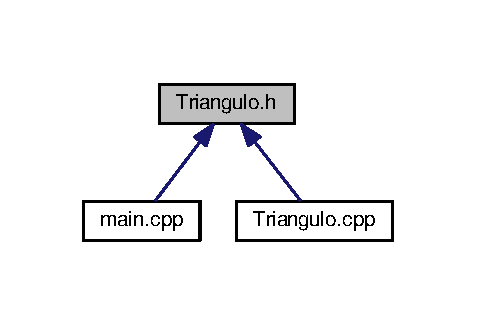
\includegraphics[width=229pt]{_triangulo_8h__dep__incl}
\end{center}
\end{figure}
\subsection*{Classes}
\begin{DoxyCompactItemize}
\item 
class \hyperlink{class_triangulo}{Triangulo}
\end{DoxyCompactItemize}

%--- End generated contents ---

% Index
\newpage
\phantomsection
\addcontentsline{toc}{chapter}{Index}
\printindex

\end{document}
